\chapter{Gameplay} 

	\section{Objective}
		\par The main goal is \textbf{SURVIVING}: away from the \textbf{forest} and back to \textbf{civilization}.
		
		\subsection{Environment}
			\par The \textbf{player} starts the game and immediately gets bombarded with \textbf{information} about its surroundings. At the \textbf{Pike Lake}, in the \textbf{middle of the woods}, \textbf{early afternoon}, during \textbf{heavy rain} that has covered the car tire tracks...with no easy way out in sight. It has no choice but to find a way to \textbf{survive}. 
			\par The \textbf{time, day, location, status bars, weather} and \textbf{remaining miles} to safety are visible on the \textbf{main screen}, ready for strategy planning.
			
		\subsection{Time}
			\par The \textbf{game time} is \underline{one hour} for every \underline{3 real minutes}. Instant actions such as \textbf{sleeping, travelling, crafting} and \textbf{exploring} take \underline{2 seconds} for any specified amount of time required for them. 
			\par The game is designed to offer the player enough time to \textbf{think, strategise} or \textbf{peruse} the inventory while taking no time in \textbf{advancing} the \textbf{story line}. Just like chess, an advanced \textbf{"speedrun"} can be completed in \underline{5 minutes}, while a \textbf{thought-out}(but poorly played) round can take up \underline{one hour and a half} with no bore or frustration from the player.
		
		\subsection{Weather}
				\par At the beginning, the \textbf{main character} is secluded by \textbf{rain}. The screen displays a ".gif" raindrop file and any action away from the car can swiftly lead to an \textbf{abrupt ending}. The car acts as a \textbf{shelter} that allows the game to still \textbf{start strong} and create the sense of urgency in order to set the \textbf{mechanics, objectives} and \textbf{priorities} for the player. 
			\par The lake is the \textbf{only} location that completely removes the \textbf{body heat depletion}. After leaving the lake,\textbf{ rain} will be the worst enemy against avoiding hypothermia and death. The user will learn that \textbf{sleeping} with surrounding warmth and \textbf{preparing for travelling} the next day is the best way to spend the night. Another tutorial-like benefit is showcasing that \textbf{clean, safe water} can be collected using a \textbf{raincatcher}, while the locations' existing sources are \textbf{dirty}.
			\par The \textbf{weather} also acts as an incentive to \textbf{explore} the very first day, which serves many purposes: teaching the \textbf{mechanic}, showing that \textbf{resources} are \textbf{not limited}, exemplifying the \textbf{status bar loss} during actions and making the player realize that Pike Lake \textbf{resources} are exclusive to it and extremely \textbf{important} to have for the rest of the \textbf{gameplay}. A \textbf{raining session} is anywhere between \underline{8} and \underline{72 hours}. The \textbf{cool down} is \underline{5} to \underline{24 hours}.
		
		\subsection{Day Time}
			\par The best time to \textbf{travel} and execute any \textbf{action} away from the current base is while it's \textbf{sunny}. There are \textbf{24 hours} in a game day, \underline{12} of daylight of \underline{12} with darkness.
			\par The player \textbf{can't see} the next possible \textbf{travel locations} without a \textbf{flashlight}. Trying to \textbf{explore, collect wood} and \textbf{set traps} will mainly result in \textbf{failure}. A flashlight can only be obtained while exploring at the Pike Lake. The item can \textbf{never} be found again after that and may even \textbf{break}.
			\par \textbf{Heat} depletes rapidly at \textbf{night}, especially during \textbf{rain}, a combination that will mostly result in game \textbf{loss}. The best night strategies are keeping a \textbf{lit fire, sleeping, crafting,} using \textbf{inventory items} and \textbf{planning to take off} first thing in the morning. 
		
		\subsection{Shelter}
			\par There is \textbf{warmth} from the \textbf{car} at the beginning of the game. Future locations require \textbf{fire} to at least stop the \textbf{heat} from dropping, which is next to that area's \textbf{place of rest} and \textbf{settlement}, also known as the \textbf{shelter}.
			\par The player may \textbf{sleep} the nights away or \textbf{build a raincatcher} from a \textbf{trash bag} in order collect \textbf{clean water}.

		\subsection{Locations}
			\par The \textbf{initial location} of the player is at \textbf{Pike Lake}. If it travels, it can \textbf{never return} again, as it is headed to the main \textbf{road}, in the opposite direction. 
			\par There are \underline{5} other \textbf{location types}(\textit{Table 2.1}) that serve as an \textbf{environment template}. The \textbf{player} may encounter the same kind of area \textbf{multiple times}, each with different faults and benefits. One may offer \textbf{water, certain resources} and \textbf{animals}, while the \textbf{road} to another could be \textbf{walked faster}.
			\begin{longtable}{|C{7em}|C{4.3em}|C{4.3em}|C{4.3em}|C{4.3em}|C{3.7em}|C{5em}|}
			   \toprule
			   \rowcolor[rgb]{ .647,  .647,  .647} \textcolor[rgb]{ 1,  1,  1}{\textbf{Locations}} & \cellcolor[rgb]{ .859,  .859,  .859}\textbf{Pike Lake} & \cellcolor[rgb]{ .859,  .859,  .859}\textbf{Flooded Area} & \cellcolor[rgb]{ .859,  .859,  .859}\textbf{Muddy Road} & \cellcolor[rgb]{ .859,  .859,  .859}\textbf{Muddy Area} & \cellcolor[rgb]{ .859,  .859,  .859}\textbf{Path} & \cellcolor[rgb]{ .859,  .859,  .859}\textbf{Woodland} \\
			   \bottomrule	
			\caption{\textbf{Game Locations}}
			\end{longtable}		
		

	\section{Status Bars}
		
		\par There are \underline{4} \textbf{values} to keep an eye on: \textbf{Condition, Body Heat, Hydration} and \textbf{Calories}. All of them can go \textbf{below} \underline{0}, signifying that the player is on its last breath. \textbf{Calories} do not lead to \textbf{death}, as a person can \textbf{realistically} go weeks \textbf{without food}, but the \textbf{game ends} when any of the others reach -\underline{15\%}.  
		
		\subsection{Condition}
			\par \textbf{Condition} is a value that can be mostly \textbf{left alone}. It improves \textbf{slightly} during the day if it's not maxed out already.  Its main purpose arises in times of desperation.
			\par The \textbf{player} may find itself in a \textbf{dire situation}, with only \textbf{dirty water}, \textbf{nearing death thirst} and \textbf{no way} to swiftly \textbf{start a fire}. Drinking it would offer a way out \textbf{once or twice}(\textit{Table 2.2}), but more is mainly \textbf{luck}. \textbf{Spoiled meat} could offer the necessary \textbf{calories} to travel the \textbf{last miles} fast as to not die of thirst, \textbf{raw meat} could be near \textbf{expiring}.
			\par There is a slight \textbf{timely increase}, as well as \textbf{bandages} to fix \textbf{travel} and \textbf{hypothermia} \textbf{wounds}, but \textbf{Condition} is mostly an end game \textbf{gamble}.

			\begin{longtable}{|C{6em}|C{6em}|C{6em}|C{6em}|C{9em}|}
			   \toprule
			   \rowcolor[rgb]{ .647,  .647,  .647} \textcolor[rgb]{ 1,  1,  1}{\textbf{Item}} & \cellcolor[rgb]{ .859,  .859,  .859}\textbf{Bandages} & \cellcolor[rgb]{ .859,  .859,  .859}\textbf{Raw Meat} & \cellcolor[rgb]{ .859,  .859,  .859}\textbf{Spoiled Meat}  & \cellcolor[rgb]{ .859,  .859,  .859}\textbf{Unsafe Water Bottle}   \\
			    \midrule
			    \rowcolor[rgb]{ .647,  .647,  .647} \textcolor[rgb]{ 1,  1,  1}{\textbf{Condition}}  & \cellcolor[rgb]{ .929,  .929,  .929}\textbf{20} & \cellcolor[rgb]{ .929,  .929,  .929}\textbf{[-70, -30]} & \cellcolor[rgb]{ .929,  .929,  .929}\textbf{[-90, -50]} & \cellcolor[rgb]{ .929,  .929,  .929}\textbf{[-60, 0]} \\	
			    \bottomrule	
			\caption{\textbf{Values} of \textbf{Condition} Changing \textbf{Items}}
			\end{longtable}
		
		\subsection{Body Heat}
			\par There are \underline{5} factors that influence \textbf{heat depletion}: \textbf{Shelter}(S), \textbf{Rain}(R), \textbf{Day Time}(D), \textbf{Clothing}(C) and \textbf{Fire}(F). 
			\par If the current location is \textbf{Pike Lake}, the player only \textbf{loses heat} if it \textbf{explores} or \textbf{travels}. That is the \textbf{only} time \textbf{shelter} is available. It can be \textbf{raining}, it can be \textbf{day or night} and the \textbf{fire} can be \textbf{lit} or not. The player \textbf{starts off} with a set of \textbf{clothing}, but it can be torn for \textbf{pieces of cloth}.
			\par The \textbf{table} below(\textit{Table 2.3}) shows all the remaining \textbf{factor combinations} and the \textbf{values} they influence \textbf{Body Heat} with every \textbf{hour}. Each \underline{"N"} preceding a factor \textbf{letter}(mentioned above) signifies \textbf{"not"}, so \underline{"NS"} would be no shelter. The code \textbf{"NSRNDCF"} reads as "\textbf{no shelter, rain, no day}(night)\textbf{, clothing}(player has it)\textbf{, fire}(is lit)" and depletes \textbf{heat} by \underline{-3} for each \textbf{hour} that the game is in that state.
			

		\begin{longtable}{|C{8em}|C{8em}|C{8em}|C{8em}|}
			   \toprule
			    \rowcolor[rgb]{ .851,  .851,  .851} \textbf{NSRDCF} & \cellcolor[rgb]{ .929,  .929,  .929}\textbf{NSNRDCF} & \textbf{NSRNDCF} & \cellcolor[rgb]{ .929,  .929,  .929}\textbf{NSRDNCF} \\
			    \midrule
			    \rowcolor[rgb]{ .851,  .851,  .851} \textbf{-2} & \cellcolor[rgb]{ .929,  .929,  .929}\textbf{30} & \textbf{-3} & \cellcolor[rgb]{ .929,  .929,  .929}\textbf{-4,5} \\
			    \midrule
			    \rowcolor[rgb]{ .929,  .929,  .929} \textbf{NSRDCNF} & \cellcolor[rgb]{ .851,  .851,  .851}\textbf{NSNRNDCF} & \textbf{NSNRDNCF} & \cellcolor[rgb]{ .749,  .749,  .749}\textbf{NSNRDCNF} \\
			    \midrule
			    \rowcolor[rgb]{ .929,  .929,  .929} \textbf{-3,5} & \cellcolor[rgb]{ .851,  .851,  .851}\textbf{25} & \textbf{28} & \cellcolor[rgb]{ .749,  .749,  .749}\textbf{0,5} \\
			    \midrule
			    \rowcolor[rgb]{ .851,  .851,  .851} \textbf{NSRNDNCF} & \cellcolor[rgb]{ .929,  .929,  .929}\textbf{NSRNDCNF} & \textbf{NSRDNCNF} & \cellcolor[rgb]{ .929,  .929,  .929}\textbf{NSNRNDNCF} \\
			    \midrule
			    \rowcolor[rgb]{ .851,  .851,  .851} \textbf{-4,5} & \cellcolor[rgb]{ .929,  .929,  .929}\textbf{-8} & \textbf{-6} & \cellcolor[rgb]{ .929,  .929,  .929}\textbf{23} \\
			    \midrule
			    \rowcolor[rgb]{ .929,  .929,  .929} \textbf{NSNRNDCNF} & \cellcolor[rgb]{ .851,  .851,  .851}\textbf{NSNRDNCNF} & \textbf{NSRNDNCNF} & \cellcolor[rgb]{ .851,  .851,  .851}\textbf{NSNRNDNCNF} \\
			    \midrule
			    \rowcolor[rgb]{ .929,  .929,  .929} \textbf{-4,5} & \cellcolor[rgb]{ .851,  .851,  .851}\textbf{0} & \textbf{-9,5} & \cellcolor[rgb]{ .851,  .851,  .851}\textbf{-6} \\
			    \bottomrule
				\caption{Game \textbf{Hourly Heat Loss} Codes and Values}
		 \end{longtable}
		
		\subsection{Hydration}
			\par \textbf{Hydration} is the most \textbf{obvious} and \textbf{mediocre} status to look after. The player \textbf{starts} with several \textbf{bottles} of liquid and it can also collect more using \textbf{empty bottles} found at \textbf{Pike Lake}.
			\par \textbf{Building a raincatcher}, collecting from \textbf{water sources}(Pike Lake, Muddy Areas and Flooded Areas) and finding \textbf{edible berries}(\textit{Table 2.4}) exploring are the ways to \textbf{get water}.
			
			\begin{longtable}{|C{5em}|C{4em}|C{4em}|C{4em}|C{4em}|C{4em}|}
			   \toprule
			   \rowcolor[rgb]{ .647,  .647,  .647} \textcolor[rgb]{ 1,  1,  1}{\textbf{Item}} & \cellcolor[rgb]{ .859,  .859,  .859}\textbf{Safe Water Bottle} & \cellcolor[rgb]{ .859,  .859,  .859}\textbf{Unsafe Water Bottle} &\cellcolor[rgb]{ .859,  .859,  .859}\textbf{Squirrel Juice} &\cellcolor[rgb]{ .859,  .859,  .859}\textbf{Soda Bottle} & \cellcolor[rgb]{ .859,  .859,  .859}\textbf{Edible Berries}  \\
			    \midrule
			    \rowcolor[rgb]{ .647,  .647,  .647} \textcolor[rgb]{ 1,  1,  1}{\textbf{Hydration}}  & \cellcolor[rgb]{ .929,  .929,  .929}\textbf{25} & \cellcolor[rgb]{ .929,  .929,  .929}\textbf{25} & \cellcolor[rgb]{ .929,  .929,  .929}\textbf{25} & \cellcolor[rgb]{ .929,  .929,  .929}\textbf{25} & \cellcolor[rgb]{ .929,  .929,  .929}\textbf{5} \\	
			    \bottomrule	
			\caption{\textbf{Values} of \textbf{Hydtration} Changing \textbf{Items}}
			\end{longtable}

		\subsection{Calories}
			\par The player \textbf{can't die} from \textbf{calorie loss}, but they are needed for \textbf{travelling}, as going below \underline{400} adds \underline{2} \textbf{extra hours} to the \textbf{length} of the journey.
			\begin{longtable}{|C{4em}|C{4em}|C{4em}|C{4em}|C{4em}|C{4em}|C{4em}|}
			   \toprule
			   \rowcolor[rgb]{ .647,  .647,  .647} \textcolor[rgb]{ 1,  1,  1}{\textbf{Item}} & \cellcolor[rgb]{ .859,  .859,  .859}\textbf{Energy Bar} &\cellcolor[rgb]{ .859,  .859,  .859}\textbf{Crickets} &\cellcolor[rgb]{ .859,  .859,  .859}\textbf{Maggots} &\cellcolor[rgb]{ .859,  .859,  .859}\textbf{Soda Bottle} & \cellcolor[rgb]{ .859,  .859,  .859}\textbf{Edible Berries} & \cellcolor[rgb]{ .859,  .859,  .859}\textbf{Squirrel Juice}  \\
			    \midrule
			    \rowcolor[rgb]{ .647,  .647,  .647} \textcolor[rgb]{ 1,  1,  1}{\textbf{Calories}} & \cellcolor[rgb]{ .929,  .929,  .929}\textbf{150} & \cellcolor[rgb]{ .929,  .929,  .929}\textbf{100} & \cellcolor[rgb]{ .929,  .929,  .929}\textbf{50} & \cellcolor[rgb]{ .929,  .929,  .929}\textbf{300} & \cellcolor[rgb]{ .929,  .929,  .929}\textbf{100} & \cellcolor[rgb]{ .929,  .929,  .929}\textbf{100}  \\	
			    \bottomrule	
			\caption{A. \textbf{Values} of \textbf{Calorie} Changing \textbf{Items}}
			\end{longtable}

			\begin{longtable}{|C{4em}|C{4em}|C{4em}|C{4em}|C{4em}|C{4em}|C{4em}|}
			   \toprule
			   \rowcolor[rgb]{ .647,  .647,  .647} \textcolor[rgb]{ 1,  1,  1}{\textbf{Item}} & \cellcolor[rgb]{ .859,  .859,  .859}\textbf{Smoked Jerky} & \cellcolor[rgb]{ .859,  .859,  .859}\textbf{Can of Peas} &\cellcolor[rgb]{ .859,  .859,  .859}\textbf{Edible Plant Part} &\cellcolor[rgb]{ .859,  .859,  .859}\textbf{Raw Meat} & \cellcolor[rgb]{ .859,  .859,  .859}\textbf{Spoiled Meat} & \cellcolor[rgb]{ .859,  .859,  .859}\textbf{Cooked Meat} \\
			    \midrule
			    \rowcolor[rgb]{ .647,  .647,  .647} \textcolor[rgb]{ 1,  1,  1}{\textbf{Calories}}  & \cellcolor[rgb]{ .929,  .929,  .929}\textbf{300} & \cellcolor[rgb]{ .929,  .929,  .929}\textbf{300} & \cellcolor[rgb]{ .929,  .929,  .929}\textbf{50} & \cellcolor[rgb]{ .929,  .929,  .929}\textbf{400} & \cellcolor[rgb]{ .929,  .929,  .929}\textbf{200} & \cellcolor[rgb]{ .929,  .929,  .929}\textbf{800} \\	
			    \bottomrule		
			\caption{B. \textbf{Values} of \textbf{Calorie} Changing \textbf{Items}}
			\end{longtable}


	\section{Inventory}
		\par The \textbf{Inventory} has a \textbf{space}(not weight) \textbf{capacity} that be increased with \textbf{extra carry items} that are crafted or owned from the beggining.  If the \textbf{space limit} is \textbf{exceeded}, then the player \textbf{can't travel}.
		\par There are \textbf{interesting ways} of going around this, such as \textbf{throwing stuff out}(the cellphone is useless and take 1 space point), crafting \textbf{compact items} from more voluminous ones(Wood Bundles), crafting \textbf{carry items}(Rope Net Bag, Pouch) and keeping \textbf{destructibles} \textbf{intact} until the \textbf{resulting resources} are needed, as they usually take \textbf{more space}. 

		\subsection{Items}
			\par The \textbf{Inventory} holds all of the player's \textbf{items} and allows their \textbf{manipulation}(Eating, Drinking, Throwing Out, Destruction). 
			\par There are \underline{5} categories: \textbf{All}(A), \textbf{Gear}(G), \textbf{Fire}(Fi), \textbf{Food}(Fo) and \textbf{Water}(Wa) for \textbf{easy navigation}, as seen in Table 2.7.

			\begin{longtable}{|C{10.555em}|C{4.0em}|C{4.0em}|C{6.445em}|C{11.055em}|}
			    \toprule
			    \rowcolor[rgb]{ .647,  .647,  .647} \textcolor[rgb]{ 1,  1,  1}{\textbf{Item}} & \textcolor[rgb]{ 1,  1,  1}{\textbf{Space}} & \textcolor[rgb]{ 1,  1,  1}{\textbf{Throw }} & \textcolor[rgb]{ 1,  1,  1}{\textbf{Category}} & \textcolor[rgb]{ 1,  1,  1}{\textbf{Items Obtained From Destruction}} \\
			    \midrule
			    \rowcolor[rgb]{ .859,  .859,  .859} \textbf{Area Map} & \textbf{0.0} & \textbf{Yes} & \textbf{A, G, Fi} & \textbf{Tinder} \\
			    \midrule
			    \rowcolor[rgb]{ .929,  .929,  .929} \textbf{Backside Of A Paper} & \textbf{1.0} & \textbf{Yes} & \textbf{A, G} & \textbf{Tinder} \\
			    \midrule
			    \rowcolor[rgb]{ .859,  .859,  .859} \textbf{Bait} & \textbf{0.34} & \textbf{Yes} & \textbf{A, G} & \textbf{-} \\
			    \midrule
			    \rowcolor[rgb]{ .929,  .929,  .929} \textbf{Bandages} & \textbf{1.0} & \textbf{Yes} & \textbf{A, G} & \textbf{Tinder} \\
			    \midrule
			    \rowcolor[rgb]{ .859,  .859,  .859} \textbf{Basic Clothes} & \textbf{0.0} & \textbf{No} & \textbf{A, G} & \textbf{Piece of Cloth, Torn Clothes} \\
			    \midrule
			    \rowcolor[rgb]{ .929,  .929,  .929} \textbf{Birch Bark} & \textbf{1.0} & \textbf{Yes} & \textbf{A, Fi} & \textbf{Tinder} \\
			    \midrule
			    \rowcolor[rgb]{ .859,  .859,  .859} \textbf{Bow Drill} & \textbf{2.0} & \textbf{Yes} & \textbf{A, Fi} & \textbf{-} \\
			    \midrule
			    \rowcolor[rgb]{ .929,  .929,  .929} \textbf{Broken Cellphone} & \textbf{1.0} & \textbf{Yes} & \textbf{A, G} & \textbf{-} \\
			    \midrule
			    \rowcolor[rgb]{ .859,  .859,  .859} \textbf{Can of Peas} & \textbf{1.0} & \textbf{Yes} & \textbf{A, Fo} & \textbf{-} \\
			    \midrule
			    \rowcolor[rgb]{ .929,  .929,  .929} \textbf{Cattail Plant} & \textbf{1.0} & \textbf{Yes} & \textbf{A, Fo} & \textbf{Edible Plant Part, Plant Fiber, Tinder} \\
			    \midrule
			    \rowcolor[rgb]{ .859,  .859,  .859} \textbf{Cooked Meat} & \textbf{1.0} & \textbf{Yes} & \textbf{A, Fo} & \textbf{-} \\
			    \midrule
			    \rowcolor[rgb]{ .929,  .929,  .929} \textbf{Crickets} & \textbf{0.34} & \textbf{Yes} & \textbf{A, Fo} & \textbf{Bait} \\
			    \midrule
			    \rowcolor[rgb]{ .859,  .859,  .859} \textbf{Dead Bird} & \textbf{3.0} & \textbf{Yes} & \textbf{A, Fo} & \textbf{Raw Meat} \\
			    \midrule
			    \rowcolor[rgb]{ .929,  .929,  .929} \textbf{Dead Fish} & \textbf{1.0} & \textbf{Yes} & \textbf{A, Fo} & \textbf{Raw Meat} \\
			    \midrule
			    \rowcolor[rgb]{ .859,  .859,  .859} \textbf{Dead Hare} & \textbf{4.0} & \textbf{Yes} & \textbf{A, Fo} & \textbf{Raw Meat, Bait, Hare Skin} \\
			    \midrule
			    \rowcolor[rgb]{ .929,  .929,  .929} \textbf{Dry Sack} & \textbf{0.0} & \textbf{Yes} & \textbf{A, G} & \textbf{-} \\
			    \midrule
			    \rowcolor[rgb]{ .859,  .859,  .859} \textbf{Duct Tape} & \textbf{0.0} & \textbf{Yes} & \textbf{A, G} & \textbf{Rope} \\
			    \midrule
			    \rowcolor[rgb]{ .929,  .929,  .929} \textbf{Edible Berries} & \textbf{1.0} & \textbf{Yes} & \textbf{A, Fo, Wa} & \textbf{Bait} \\
			    \midrule
			    \rowcolor[rgb]{ .859,  .859,  .859} \textbf{Edible Plant Part} & \textbf{1.0} & \textbf{Yes} & \textbf{A, Fo} & \textbf{-} \\
			    \midrule
			    \rowcolor[rgb]{ .929,  .929,  .929} \textbf{Empty Bottle} & \textbf{1.0} & \textbf{Yes} & \textbf{A, Wa} & \textbf{-} \\
			    \midrule
			    \rowcolor[rgb]{ .859,  .859,  .859} \textbf{Empty Can} & \textbf{0.0} & \textbf{No} & \textbf{A, G} & \textbf{-} \\
			    \midrule
			    \rowcolor[rgb]{ .929,  .929,  .929} \textbf{Energy Bar} & \textbf{0.0} & \textbf{No} & \textbf{A, Fo} & \textbf{Bait} \\
			    \midrule
			    \rowcolor[rgb]{ .859,  .859,  .859} \textbf{Fire Plow} & \textbf{1.0} & \textbf{Yes} & \textbf{A, Fi} & \textbf{-} \\
			    \midrule
			    \rowcolor[rgb]{ .929,  .929,  .929} \textbf{First Aid Kit} & \textbf{2.0} & \textbf{Yes} & \textbf{A, G} & \textbf{First Aid Book, Bandages, Pouch} \\
			    \midrule
			    \rowcolor[rgb]{ .859,  .859,  .859} \textbf{First Aid Manual} & \textbf{1.0} & \textbf{Yes} & \textbf{A, G} & \textbf{Backside of Paper} \\
			    \midrule
			    \rowcolor[rgb]{ .929,  .929,  .929} \textbf{Fishing Hook} & \textbf{0.34} & \textbf{Yes} & \textbf{A, G} & \textbf{-} \\
			    \midrule
			    \rowcolor[rgb]{ .859,  .859,  .859} \textbf{Fishing Kit} & \textbf{2.0} & \textbf{Yes} & \textbf{A, G} & \textbf{Empty Can, Rope, Fishing Hook} \\
			    \midrule
			    \rowcolor[rgb]{ .929,  .929,  .929} \textbf{Fishing Rod} & \textbf{3.0} & \textbf{Yes} & \textbf{A, G} & \textbf{Wood, Rope, Fishing Hook} \\
			    \midrule
			    \rowcolor[rgb]{ .859,  .859,  .859} \textbf{Flashlight} & \textbf{2.0} & \textbf{Yes} & \textbf{A, G} & \textbf{-} \\
			    \midrule
			    \rowcolor[rgb]{ .929,  .929,  .929} \textbf{Hardwood} & \textbf{4.0} & \textbf{Yes} & \textbf{A, Fi} & \textbf{Wood} \\
			    \midrule
			    \rowcolor[rgb]{ .859,  .859,  .859} \textbf{Hare Skin} & \textbf{1.0} & \textbf{Yes} & \textbf{A, G} & \textbf{-} \\
			    \midrule
			    \rowcolor[rgb]{ .929,  .929,  .929} \textbf{Knife} & \textbf{0.0} & \textbf{No} & \textbf{A, G} & \textbf{-} \\
			    \midrule
			    \rowcolor[rgb]{ .859,  .859,  .859} \textbf{Maggots} & \textbf{0.34} & \textbf{Yes} & \textbf{A, Fo} & \textbf{Bait} \\
			    \midrule
			    \rowcolor[rgb]{ .929,  .929,  .929} \textbf{Matches} & \textbf{0.0} & \textbf{Yes} & \textbf{A, Fi} & \textbf{-} \\
			    \midrule
			    \rowcolor[rgb]{ .859,  .859,  .859} \textbf{Newspaper} & \textbf{1.0} & \textbf{Yes} & \textbf{A, G} & \textbf{Tinder} \\
			    \midrule
			    \rowcolor[rgb]{ .929,  .929,  .929} \textbf{Piece of Cloth} & \textbf{1.0} & \textbf{Yes} & \textbf{A, G} & \textbf{Bandages} \\
			    \midrule
			    \rowcolor[rgb]{ .859,  .859,  .859} \textbf{Plant Fiber} & \textbf{1.0} & \textbf{Yes} & \textbf{A, G} & \textbf{Rope} \\
			    \midrule
			    \rowcolor[rgb]{ .929,  .929,  .929} \textbf{Pouch} & \textbf{0.0} & \textbf{No} & \textbf{A, G} & \textbf{-} \\
			    \midrule
			    \rowcolor[rgb]{ .859,  .859,  .859} \textbf{Raw Meat} & \textbf{1.0} & \textbf{Yes} & \textbf{A, Fo} & \textbf{Bait} \\
			    \midrule
			    \rowcolor[rgb]{ .929,  .929,  .929} \textbf{Rope} & \textbf{0.34} & \textbf{Yes} & \textbf{A, G} & \textbf{-} \\
			    \midrule
			    \rowcolor[rgb]{ .859,  .859,  .859} \textbf{Rope Net Bag} & \textbf{0.0} & \textbf{Yes} & \textbf{A, G} & \textbf{-} \\
			    \midrule
			    \rowcolor[rgb]{ .929,  .929,  .929} \textbf{Safe Water Bottle} & \textbf{2.0} & \textbf{No} & \textbf{A, Wa} & \textbf{Empty Bottle} \\
			    \midrule
			    \rowcolor[rgb]{ .859,  .859,  .859} \textbf{Smoked Jerky} & \textbf{1.0} & \textbf{No} & \textbf{A, Fo} & \textbf{Bait} \\
			    \midrule
			    \rowcolor[rgb]{ .929,  .929,  .929} \textbf{Soda Bottle} & \textbf{2.0} & \textbf{No} & \textbf{A, Fo, Wa} & \textbf{Empty Bottle} \\
			    \midrule
			    \rowcolor[rgb]{ .859,  .859,  .859} \textbf{Spoiled Meat} & \textbf{3.0} & \textbf{Yes} & \textbf{A, Fo} & \textbf{-} \\
			    \midrule
			    \rowcolor[rgb]{ .929,  .929,  .929} \textbf{Squirrel Juice} & \textbf{1.0} & \textbf{No} & \textbf{A, Fo, Wa} & \textbf{Empty Bottle} \\
			    \midrule
			    \rowcolor[rgb]{ .859,  .859,  .859} \textbf{Tinder} & \textbf{0.34} & \textbf{Yes} & \textbf{A, Fi} & \textbf{-} \\
			    \midrule
			    \rowcolor[rgb]{ .929,  .929,  .929} \textbf{Torn Clothes} & \textbf{0.0} & \textbf{No} & \textbf{A, G} & \textbf{-} \\
			    \midrule
			    \rowcolor[rgb]{ .859,  .859,  .859} \textbf{Trash Bag} & \textbf{0.0} & \textbf{Yes} & \textbf{A, G} & \textbf{Rope} \\
			    \midrule
			    \rowcolor[rgb]{ .929,  .929,  .929} \textbf{Unsafe Water Bottle} & \textbf{2.0} & \textbf{No} & \textbf{A, Wa} & \textbf{Empty Bottle} \\
			    \midrule
			    \rowcolor[rgb]{ .859,  .859,  .859} \textbf{Utility Belt Bag} & \textbf{0.0} & \textbf{Yes} & \textbf{A, G} & \textbf{-} \\
			    \midrule
			    \rowcolor[rgb]{ .929,  .929,  .929} \textbf{Wires} & \textbf{0.34} & \textbf{Yes} & \textbf{A, G} & \textbf{Rope} \\
			    \midrule
			    \rowcolor[rgb]{ .859,  .859,  .859} \textbf{Wood} & \textbf{3.0} & \textbf{Yes} & \textbf{A, Fi} & \textbf{Tinder} \\
			    \midrule
			    \rowcolor[rgb]{ .929,  .929,  .929} \textbf{Wood Bundle} & \textbf{6.0} & \textbf{Yes} & \textbf{A, Fi} & \textbf{Wood} \\
			    \midrule
			    \rowcolor[rgb]{ .859,  .859,  .859} \textbf{Wooden Spear} & \textbf{1.0} & \textbf{Yes} & \textbf{A, G} & \textbf{Wood} \\
			    \bottomrule
			\caption{\textbf{Inventory Items}}
			\end{longtable}


		\subsection{Spoilage}
			\par There are certain \textbf{items}(\textit{Table 2.8}) that can \textbf{spoil}. \textbf{Trap prey} only lasts a \textbf{couple of hours} after \textbf{death}, when it turns into \textbf{Spoiled Meat}. 
			\par The only meat \textbf{preservation} method is drying it at the \textbf{fire} to make \textbf{Smoked Jerky}.

			\begin{longtable}{|C{10.555em}|C{4.0em}|C{4.0em}|C{4.0em}|C{4.0em}|C{4.0em}|}
			    \toprule
			    \rowcolor[rgb]{ .647,  .647,  .647} \textcolor[rgb]{ 1,  1,  1}{\textbf{Item}} &\cellcolor[rgb]{ .859,  .859,  .859}\textbf{Raw Meat} &\cellcolor[rgb]{ .859,  .859,  .859}\textbf{Cooked Meat} & \cellcolor[rgb]{ .859,  .859,  .859}\textbf{Dead Hare} & \cellcolor[rgb]{ .859,  .859,  .859}\textbf{Dead Fish} & \cellcolor[rgb]{ .859,  .859,  .859}\textbf{Dead Bird} \\
			    \midrule
			    \rowcolor[rgb]{ .647,  .647,  .647} \textcolor[rgb]{ 1,  1,  1}{\textbf{Hours Until Spoilage}} & \cellcolor[rgb]{ .929,  .929,  .929}\textbf{15} & \cellcolor[rgb]{ .929,  .929,  .929}\textbf{24} & \cellcolor[rgb]{ .929,  .929,  .929}\textbf{24} & \cellcolor[rgb]{ .929,  .929,  .929}\textbf{8} & \cellcolor[rgb]{ .929,  .929,  .929}\textbf{14} \\
			    \bottomrule	
			\caption{\textbf{\textbf{Items} That \textbf{Spoil} and \textbf{Freshness Durations}}}
			\end{longtable}


	\section{Fire}
		\par The \textbf{fire} screen has the most \textbf{complex} process from the \textbf{player's perspective}(\textit{Figure 2.1}). It is the \textbf{best asset} against \textbf{rain} and \textbf{night temperatures}.
		\par The \textbf{best strategy} is collecting \textbf{wood} during the \textbf{day} and using it to start a \textbf{fire} at \textbf{night}, when the player can \textbf{sleep} or \textbf{prepare} to go to the \textbf{next location} at dawn. 
		\par \textbf{Fire} allows for \textbf{water boiling} and \textbf{meat processing}, such a \textbf{cooking} and \textbf{drying} to avoid \textbf{Condition loss}.
		\par There needs to be \textbf{tinder} and one type of \textbf{tool} to \textbf{start a fire}. It is \textbf{maintained} with \textbf{tinder, wood} or \textbf{hardwood}. 

		\subsection{Fire Starting}
			\par The \textbf{fire starting tools}(\textit{Table 2.9}) have a fire starting \textbf{success rate}(the \textbf{Matches} work \underline{all the time}, the \textbf{Fire Plow} works in \underline{30\%} of the \textbf{cases}). They can also be \textbf{destroyed} while being used(the \textbf{Matches} are \underline{completely used up}, the \textbf{Bow Drill} has a \underline{3\%} chance of \textbf{breaking}).
			\begin{longtable}{|C{7em}|C{7em}|C{12em}|}
			   \toprule
			  \rowcolor[rgb]{ .647,  .647,  .647} \textcolor[rgb]{ 1,  1,  1}{\textbf{Fire Tools}} & \textcolor[rgb]{ 1,  1,  1}{\textbf{Success Rate}} & \textcolor[rgb]{ 1,  1,  1}{\textbf{Destruction Rate}} \\
			    \midrule
			    \rowcolor[rgb]{ .859,  .859,  .859} \textbf{Matches} & \textbf{100\%} & \textbf{100\%} \\
			    \midrule
			    \rowcolor[rgb]{ .929,  .929,  .929} \textbf{Bow Drill} & \textbf{50\%} & \textbf{3\%} \\
			    \midrule
			    \rowcolor[rgb]{ .859,  .859,  .859} \textbf{Fire Plow} & \textbf{30\%} & \textbf{6\%} \\
			    \bottomrule	
			\caption{\textbf{\textbf{Fire} starting \textbf{Tools} and \textbf{Quality}}}
			\end{longtable}

		\begin{figure}[H]
			\centering
			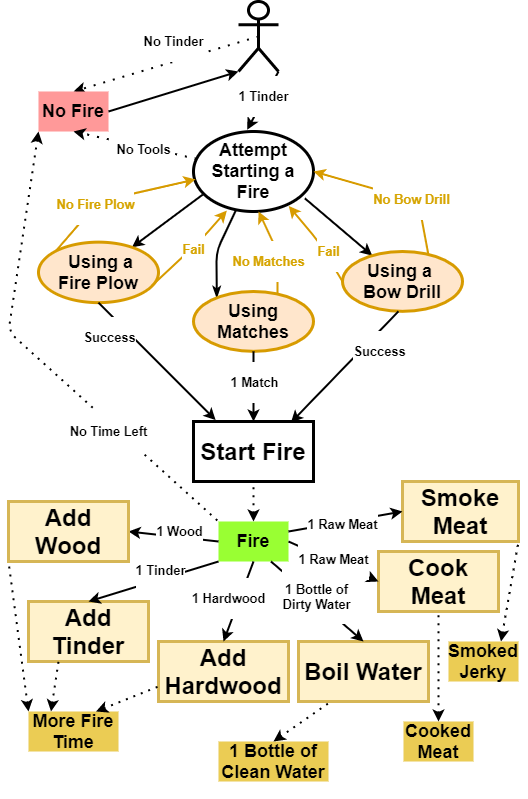
\includegraphics[width=15cm, height=17cm, keepaspectratio]{Images/FireUseCase.png}\\
			\caption{\textbf{Fire Screen Process}}
		\end{figure}


\section{Crafting}
		\par Creating \textbf{complex} items is displayed as \textbf{crafting}, while \textbf{breaking} them apart to get \textbf{parts} can be done in the \textbf{inventory}. Making something new takes \textbf{time} and \textbf{place} near the \textbf{fire}, so it can be done at \textbf{night} with no \textbf{Body Heat loss}.
		\par The \textbf{table} below(\textit{Table 2.10}) showcases all the \textbf{items} that can be \textbf{created}, the \textbf{time} needed, the \textbf{resources} and their \textbf{descriptions}. There can \textbf{only} be \textbf{one} of a certain device in the \textbf{inventory}(Fire Plow, Bow Drill).
		\par \textbf{Crafting} can help with \textbf{Inventory Management} in many ways. There are \textbf{bags} for \textbf{extra space}(Pouch) or \textbf{creations} that are \textbf{more compact} than their \textbf{loose parts}(Wood Bundle, Rope).

		\begin{longtable}{|C{6em}|C{6em}|C{8em}|C{17em}|}
		   \toprule
		   \rowcolor[rgb]{ .647,  .647,  .647} \textcolor[rgb]{ 1,  1,  1}{\textbf{Item}} & \textcolor[rgb]{ 1,  1,  1}{\textbf{Crafting Duration}} & \textcolor[rgb]{ 1,  1,  1}{\textbf{Crafting Resources}} & \textcolor[rgb]{ 1,  1,  1}{\textbf{Description}} \\
		    \midrule
		    \rowcolor[rgb]{ .859,  .859,  .859} \textbf{Fire Plow} & \textbf{30 minutes} & \textbf{Wood} & \textbf{"A primitive tool for starting a fire. Rubbing two sticks together should produce an ember. I can only have one."} \\
		    \midrule
		    \rowcolor[rgb]{ .929,  .929,  .929} \textbf{Bow Drill} & \textbf{30 minutes} & \textbf{Rope, Hardwood} & \textbf{"A primitive tool for starting a fire. Using the bow drill requires some skill and plenty of patience. I can only have one."} \\
		    \midrule
		    \rowcolor[rgb]{ .859,  .859,  .859} \textbf{Fishing Rod} & \textbf{30 minutes} & \textbf{2 Ropes, Fishing Hook, Wood} & \textbf{"A survival fishing rod made of stick, rope, and a hook. Good enough to catch a fish. I can only have one."} \\
		    \midrule
		    \rowcolor[rgb]{ .929,  .929,  .929} \textbf{Wooden Fishing Hook} & \textbf{60 minutes} & \textbf{Wood} & \textbf{"A fishing hook. Sharp end."} \\
		    \midrule
		    \rowcolor[rgb]{ .859,  .859,  .859} \textbf{Rope} & \textbf{30 minutes} & \textbf{Piece Of Cloth} & \textbf{"Piece of rope. Useful for many purposes in a survival situation. Each piece of rope requires 1/3 unit of carry space."} \\
		    \midrule
		    \rowcolor[rgb]{ .929,  .929,  .929} \textbf{Wooden Spear} & \textbf{30 minutes} & \textbf{Hardwood} & \textbf{"It's a wooden spear with a pretty sharp tip. Better than bare handed hunting. I can only have one."} \\
		    \midrule
		    \rowcolor[rgb]{ .859,  .859,  .859} \textbf{Rope Net Bag} & \textbf{180 minutes} & \textbf{3 Ropes} & \textbf{"A survival net bag made of rope. Useful for carrying additional gear[+4 CARRY SPACE]. I can only have one."} \\
		    \midrule
		    \rowcolor[rgb]{ .929,  .929,  .929} \textbf{Pouch} & \textbf{120 minutes} & \textbf{Hare Skin, Rope} & \textbf{"A small pouch. I can carry stuff in it. I can have a couple of these.[+1 CARRY SPACE]"} \\
		    \midrule
		    \rowcolor[rgb]{ .859,  .859,  .859} \textbf{Wood Bundle} & \textbf{60 minutes} & \textbf{4 Woods, Rope} & \textbf{"Bunch of wood tied together. Makes it easier to carry."} \\
   		    \bottomrule	
		\caption{\textbf{Craftable Items}}
		\end{longtable}

	\section{Location Specific Actions}
		\subsection{Exploring}
			\par \textbf{Each time} the player arrives \textbf{somewhere new}, the game takes the \textbf{location type} and uses its \textbf{"Number of Resources"} interval(\textit{Table 2.11}) to \textbf{randomize} how many resources to \textbf{create}.
			\begin{longtable}{|C{7em}|C{4.3em}|C{4.3em}|C{4.3em}|C{4.3em}|C{3.7em}|C{5em}|}
			   \toprule
			   \rowcolor[rgb]{ .647,  .647,  .647} \textcolor[rgb]{ 1,  1,  1}{\textbf{Location}} & \cellcolor[rgb]{ .859,  .859,  .859}\textbf{Pike Lake} & \cellcolor[rgb]{ .859,  .859,  .859}\textbf{Flooded Area} & \cellcolor[rgb]{ .859,  .859,  .859}\textbf{Muddy Road} & \cellcolor[rgb]{ .859,  .859,  .859}\textbf{Muddy Area} & \cellcolor[rgb]{ .859,  .859,  .859}\textbf{Path} & \cellcolor[rgb]{ .859,  .859,  .859}\textbf{Woodland} \\
			   \midrule
			   \rowcolor[rgb]{ .647,  .647,  .647} \textcolor[rgb]{ 1,  1,  1}{\textbf{Number Of Resources}} & \cellcolor[rgb]{ .859,  .859,  .859}\textbf{\{3, 6\}} & \cellcolor[rgb]{ .859,  .859,  .859}\textbf{\{3, 6\}} & \cellcolor[rgb]{ .859,  .859,  .859}\textbf{\{9, 11\}} & \cellcolor[rgb]{ .859,  .859,  .859}\textbf{\{7, 9\}} & \cellcolor[rgb]{ .859,  .859,  .859}\textbf{\{8, 10\}} & \cellcolor[rgb]{ .859,  .859,  .859}\textbf{\{6, 8\}} \\
			   \bottomrule	
			\caption{\textbf{Amount} of \textbf{Resources} at a \textbf{Location Type}}
			\end{longtable}

			\par Each \textbf{location type} has some \textbf{items} and their \textbf{probability to be randomized} in the \textbf{current} place's \textbf{"Available Explorables"} list(\textit{Table 2.12}).
		        \begin{longtable}{|C{10em}|C{4.5em}|C{4.5em}|C{4.5em}|C{3.5em}|C{5em}}
			    \toprule
			    \rowcolor[rgb]{ .647,  .647,  .647} \textcolor[rgb]{ 1,  1,  1}{\textbf{Resource/Location}} & \textcolor[rgb]{ 1,  1,  1}{\textbf{Flooded Area}} & \textcolor[rgb]{ 1,  1,  1}{\textbf{Muddy Road}} & \textcolor[rgb]{ 1,  1,  1}{\textbf{Muddy Area}} & \textcolor[rgb]{ 1,  1,  1}{\textbf{Path}} & \textcolor[rgb]{ 1,  1,  1}{\textbf{Woodland}} \\
			    \midrule
			    \rowcolor[rgb]{ .859,  .859,  .859} \textbf{Wood} & \textbf{-} & \textbf{20\%} & \textbf{35\%} & \textbf{-} & \textbf{-} \\
			    \midrule
			    \rowcolor[rgb]{ .929,  .929,  .929} \textbf{Cattail Plant} & \textbf{-} & \textbf{-} & \textbf{-} & \textbf{24\%} & \textbf{28\%} \\
			    \midrule
			    \rowcolor[rgb]{ .859,  .859,  .859} \textbf{Maggots} & \textbf{17\%} & \textbf{-} & \textbf{-} & \textbf{29\%} &\textbf{38\%} \\
			    \midrule
			    \rowcolor[rgb]{ .929,  .929,  .929} \textbf{Crickets} & \textbf{} & \textbf{14\%} & \textbf{23\%} & \textbf{33\%} &\textbf{28\%} \\
			    \midrule
			    \rowcolor[rgb]{ .859,  .859,  .859} \textbf{Cattail Plant} & \textbf{45\%} & \textbf{-} &\textbf{-} & \textbf{-} & \textbf{-} \\
			    \midrule
			    \rowcolor[rgb]{ .929,  .929,  .929} \textbf{Edible Berries} & \textbf{-} & \textbf{22\%} & \textbf{12\%} & \textbf{14\%} & \textbf{6\%} \\
			    \midrule
			    \rowcolor[rgb]{ .859,  .859,  .859} \textbf{Plant Fiber} & \textbf{38\%} & \textbf{9\%} & \textbf{23\%} & \textbf{-} & \textbf{-} \\
			    \midrule
			    \rowcolor[rgb]{ .929,  .929,  .929} \textbf{Birch Bark} & \textbf{-} & \textbf{24\%} & \textbf{7\%} & \textbf{-} & \textbf{-} \\
			    \bottomrule	
			\caption{\textbf{Chance} of \textbf{Item} \textbf{Finding} at Certain \textbf{Locations}}
			\end{longtable}

			\par \textbf{Pike Lake} has some \textbf{exclusive} items that are \textbf{very useful} for the \textbf{gameplay}, as it can only be visited \textbf{once}, at the beginning.(\textit{Table 2.13}).

			\begin{longtable}{|C{2.4em}|C{3.2em}|C{3.0em}|C{3.2em}|C{3.4em}|C{2.8em}|C{3.5em}|C{4.0em}|C{4.0em}|}
			    \toprule
			    \rowcolor[rgb]{ .647,  .647,  .647} \textcolor[rgb]{ 1,  1,  1}{\textbf{Item}} & \cellcolor[rgb]{ .859,  .859,  .859}\textbf{Flash Light} & \cellcolor[rgb]{ .859,  .859,  .859}\textbf{Wires} & \cellcolor[rgb]{ .859,  .859,  .859}\textbf{Empty Bottle} & \cellcolor[rgb]{ .859,  .859,  .859}\textbf{News Paper} & \cellcolor[rgb]{ .859,  .859,  .859}\textbf{Duct Tape} & \cellcolor[rgb]{ .859,  .859,  .859}\textbf{Fishing Kit} & \cellcolor[rgb]{ .859,  .859,  .859}\textbf{Matches} & \cellcolor[rgb]{ .859,  .859,  .859}\textbf{First Aid Kit} \\
			    \midrule
			    \rowcolor[rgb]{ .647,  .647,  .647} \textcolor[rgb]{ 1,  1,  1}{\textbf{\%}} & \cellcolor[rgb]{ .929,  .929,  .929}\textbf{15\%} & \cellcolor[rgb]{ .929,  .929,  .929}\textbf{25\%} & \cellcolor[rgb]{ .929,  .929,  .929}\textbf{10\%} & \cellcolor[rgb]{ .929,  .929,  .929}\textbf{15\%} & \cellcolor[rgb]{ .929,  .929,  .929}\textbf{9\%} & \cellcolor[rgb]{ .929,  .929,  .929}\textbf{8\%} & \cellcolor[rgb]{ .929,  .929,  .929}\textbf{8\%} & \cellcolor[rgb]{ .929,  .929,  .929}\textbf{10\%} \\
			     \bottomrule	
			\caption{\textbf{Chance} of \textbf{Finding} an \textbf{Item} at \textbf{Pike Lake}}
			\end{longtable}

		\subsection{Getting Wood}
		\par \textbf{Wood} can't be collected at \textbf{Pike Lake}, in order to promote \textbf{Exploring} for \textbf{new players} and because the \textbf{car} acts as a \textbf{shelter}. There is \textbf{no limit} at any locations, the player only has the \textbf{night} without a \textbf{flaslight} to worry about.

		\subsection{Getting Water}
			\par \textbf{Clean water} can be obtained through a \textbf{raincatcher}, but \textbf{dirty water} can be collected from locations that have it as a \textbf{resource}(\textit{Table 2.14}).
			\begin{longtable}{|C{7em}|C{3.5em}|C{4.5em}|C{4.5em}|C{4.5em}|C{3.5em}|C{5em}|}
			   \toprule
			   \rowcolor[rgb]{ .647,  .647,  .647} \textcolor[rgb]{ 1,  1,  1}{\textbf{Location}} & \cellcolor[rgb]{ .859,  .859,  .859}\textbf{Pike Lake} & \cellcolor[rgb]{ .859,  .859,  .859}\textbf{Flooded Area} & \cellcolor[rgb]{ .859,  .859,  .859}\textbf{Muddy Road} & \cellcolor[rgb]{ .859,  .859,  .859}\textbf{Muddy Area} & \cellcolor[rgb]{ .859,  .859,  .859}\textbf{Path} & \cellcolor[rgb]{ .859,  .859,  .859}\textbf{Woodland} \\
			  \midrule			    
			  \rowcolor[rgb]{ .647,  .647,  .647} \textcolor[rgb]{ 1,  1,  1}{\textbf{Dirty Water Source}} & \cellcolor[rgb]{ .859,  .859,  .859}\textbf{Yes} & \cellcolor[rgb]{ .859,  .859,  .859}\textbf{Yes} & \cellcolor[rgb]{ .859,  .859,  .859}\textbf{No} & \cellcolor[rgb]{ .859,  .859,  .859}\textbf{Yes} & \cellcolor[rgb]{ .859,  .859,  .859}\textbf{No} & \cellcolor[rgb]{ .859,  .859,  .859}\textbf{No} \\
			    \bottomrule	
			\caption{\textbf{Location Types} \textbf{Water Resources}}
			\end{longtable}
		
		\subsection{Setting Traps and Catching Fish}
		
		\par \textbf{Traps} have their own \textbf{screen} that allows \textbf{building and dismantling}. The \textbf{amount} that can be made of each is  \textbf{infinite} if the resources are there, so the  \textbf{chance} gets \textbf{better} with each  \textbf{new one}(\textit{Table 2.15}). \textbf{Fish} can be caught with a \textbf{spear}(5\%) or \textbf{fished}(8\%).
			\begin{longtable}{|C{6em}|C{6em}|C{5em}|C{9em}|C{9em}|}
			   \toprule
			   \rowcolor[rgb]{ .647,  .647,  .647} \textcolor[rgb]{ 1,  1,  1}{\textbf{Traps}} & \textcolor[rgb]{ 1,  1,  1}{\textbf{Hourly Trap Rate}} & \textcolor[rgb]{ 1,  1,  1}{\textbf{Prey}} & \textcolor[rgb]{ 1,  1,  1}{\textbf{Prey Resources}} & \textcolor[rgb]{ 1,  1,  1}{\textbf{Building Resources}} \\
			    \midrule
			    \rowcolor[rgb]{ .859,  .859,  .859} \textbf{Deadfall} & \textbf{2\%} & \textbf{Hare} & \textbf{3 Raw Meats, Bait, Hare Skin} & \textbf{Rope, Wood, Bait} \\
			    \midrule
			    \rowcolor[rgb]{ .929,  .929,  .929} \textbf{Fish Trap} & \textbf{3\%} & \textbf{Fish} & \textbf{1 Raw Meat} & \textbf{Rope, Wood, Bait} \\
			    \midrule
			    \rowcolor[rgb]{ .859,  .859,  .859} \textbf{Bird Trap} & \textbf{4\%} & \textbf{Bird} & \textbf{2 Raw Meats} & \textbf{Rope, Wood, Bait} \\
			    \bottomrule
			\caption{\textbf{Traps} }	
			\end{longtable}

	\section{Travel}
		\par \textbf{Travelling} to a location requires an \textbf{inventory} below the \textbf{space threshold}. The \textbf{number} of travel hours is \textbf{randomized} from the specific \textbf{interval}. 
		\par If the player has less than \underline{400} calories, \underline{2} \textbf{extra hours} are added to the \textbf{trip}. The location \textbf{choices} are \textbf{not visible} at night without a \textbf{flashlight}(\textit{Table 2.16}).
		\begin{longtable}{|C{10.555em}|C{5.22em}|C{5.22em}|C{6.445em}|}
		    \toprule			    
		    \rowcolor[rgb]{ .647,  .647,  .647} \textcolor[rgb]{ 1,  1,  1}{\textbf{Location}} & \textcolor[rgb]{ 1,  1,  1}{\textbf{Miles}} & \textcolor[rgb]{ 1,  1,  1}{\textbf{Hours}} & \textcolor[rgb]{ 1,  1,  1}{\textbf{Water Source}} \\
		    \midrule
		    \rowcolor[rgb]{ .859,  .859,  .859} \textbf{Pike Lake} & \textbf{3} & \textbf{\{4, 5\}} & \textbf{Yes} \\
		    \midrule
		    \rowcolor[rgb]{ .929,  .929,  .929} \textbf{Flooded Area} & \textbf{2} & \textbf{\{4, 5\}} & \textbf{Yes} \\
		    \midrule
		    \rowcolor[rgb]{ .859,  .859,  .859} \textbf{Muddy Road} & \textbf{2} & \textbf{\{3, 4\}} & \textbf{No} \\
		    \midrule
		    \rowcolor[rgb]{ .929,  .929,  .929} \textbf{Muddy Area} & \textbf{2} & \textbf{\{3, 4\}} & \textbf{Yes} \\
		    \midrule
		    \rowcolor[rgb]{ .859,  .859,  .859} \textbf{Path} & \textbf{3} & \textbf{\{3, 4\}} & \textbf{No} \\
		    \midrule
		    \rowcolor[rgb]{ .929,  .929,  .929} \textbf{Woodland} & \textbf{2} & \textbf{\{3, 4\}} & \textbf{No} \\
		    \bottomrule
		\caption{\textbf{Travel Information} }	
		\end{longtable}


\newpage